\chapter*{Introduction}
\addcontentsline{toc}{chapter}{Introduction}

Introduce the problem, explain why it is interesting and outline the goal of the thesis.

%%-----------------------------------------------------------------------------------------
%% SECTION
%%-----------------------------------------------------------------------------------------
\section*{Morphome3cs}

TODO
%%-----------------------------------------------------------------------------------------
%% SECTION
%%-----------------------------------------------------------------------------------------
\section*{Applications of Mesh Difference Visualization}

TODO
%%-----------------------------------------------------------------------------------------
%% SECTION
%%-----------------------------------------------------------------------------------------
\section*{Mesh Difference Visualization in Morphome3cs and Elsewhere}

Morphome3cs is able to generate a homologous\footnotemark pair of triangle meshes from two arbitrary triangle meshes and use it to compute and visualize the difference between them. Currently, Morphome3cs is able to produce color-based visualizations of multiple difference metrics. These metrics are:

\begin{itemize}
\item Corresponding vertex distance (fig. \ref{fig:morpho_example})
\item Corresponding vertex distance projected into the surface normal
\item Angle between corresponding surface normals
\item FESA\footnotemark
\item Curvature difference
\end{itemize}

The disadvantage of these color-based visualizations is that they fail to capture multi-dimensional information. For example, when using vertex distance as a metric, it is impossible to encode both magnitude and direction into color at the same time while maintaining visual clarity.

\begin{figure}[h]
\centering
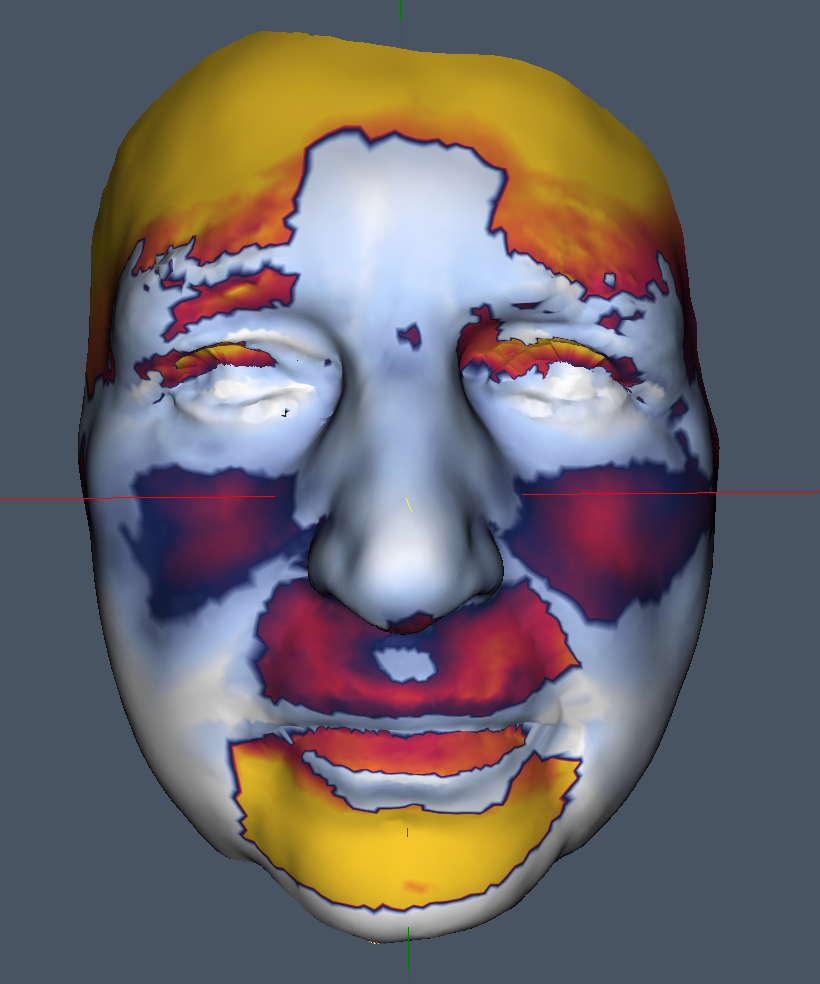
\includegraphics[width=0.5\textwidth]{./img/morpho-example01.PNG}
\caption{Morphome3cs - Vertex difference visualization}
\label{fig:morpho_example}
\end{figure}

Other approaches can be found for example in MeshLab (fig. \ref{fig:meshlab_example}) and CloudCompare (fig. \ref{fig:cloudcompare_example}). In MeshLab, the difference between two arbitrary triangle meshes can be visualized directly by using the Hausdorff Distance\footnotemark encoded into color. CloudCompare is able to visualize the difference between two arbitrary triangle meshes (or a triangle mesh and a point cloud) by simply finding the nearest triangle to a given point, computing the distance and encoding this metric into color \citep{CloudCmpDistance}. It can also produce a color-based visualization of the difference between two point clouds.

\begin{figure}[h]
\centering
	\begin{subfigure}{0.3\textwidth}
	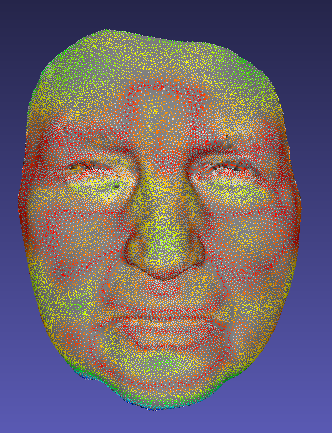
\includegraphics[width=\textwidth]{./img/meshlab-example01.PNG}
    \caption{MeshLab - Hausdorff Distance visualization}
    \label{fig:meshlab_example}
	\end{subfigure}
    \qquad
    \begin{subfigure}{0.3\textwidth}
	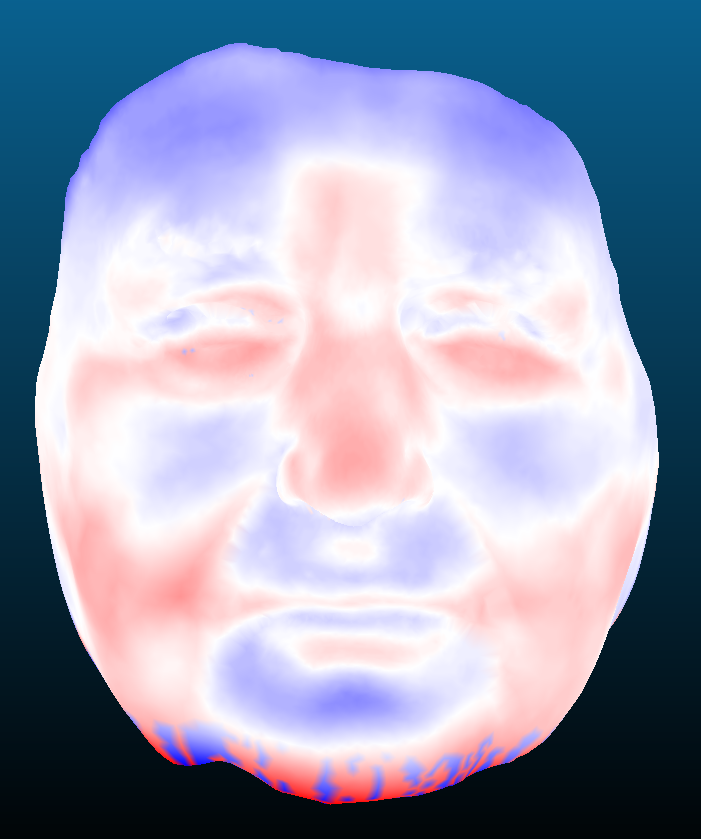
\includegraphics[width=\textwidth]{./img/cloudcompare-example01.PNG}
    \caption{CloudCompare - Vertex distance visualization}
    \label{fig:cloudcompare_example}
	\end{subfigure}
\caption{Visualizations in MeshLab and CloudCompare}
\end{figure}

\addtocounter{footnote}{-3}
\stepcounter{footnote}\footnotetext{Two triangle meshes are homologous if they have the same number of vertices and there is a one-to-one mapping between them. Vertices are numbered and vertex \(v_i \in Mesh_1\) corresponds to vertex \(v_i \in Mesh_2\).}
\stepcounter{footnote}\footnotetext{Finite Element Surface Analysis, captures the difference between corresponding triangle areas}
\stepcounter{footnote}\footnotetext{One-sided Hausdorff Distance between two point sets \(S_1, S_2\) is defined as \(E(S_1, S_2) = \max_{p \in S_1} \min_{p' \in S_2} d(p, p')\) where \(d\) is the Euclidean distance between two points. Details of the computation used in MeshLab can be found in \citet{Metro98}.}
%%-----------------------------------------------------------------------------------------
%% SECTION
%%-----------------------------------------------------------------------------------------
\section*{Our Goal}

In order to overcome the limitations of the above color-based visualizations, this thesis is looking to create arrow-based visualizations which will be able to display multidimensional information. We will visualize difference metrics from Morphome3cs which are suitable for such visualizations, namely {\it corresponding vertex distance} and {\it corresponding vertex distance projected into the surface normal}. The input of our algorithm will be homologous triangle meshes as in Morphome3cs. We will focus on the visual appearance of devised visualizations and their implementation in an experimental application called MeshDiff. Lastly, a user study will be carried out to assess the quality of the new visualizations in various use cases. This study will serve as a basis for further development and potential incorporation of the visualizations into Morphome3cs.
%%-----------------------------------------------------------------------------------------
%% SECTION
%%-----------------------------------------------------------------------------------------
\section*{Thesis Structure}

Chpater 1 of this thesis is concerned with the description of the proposed visualizations and the main ideas behind them. Chapter 2 delves into the implementation details of the visualizations in MeshDiff. Chapter 3 provides a user documentation of MeshDiff and Chapter 4 presents the results of the user study.